\documentclass[main.tex]{subfiles} % Subfile-Class


% ============================================================================== %
%                            Subfile document                                    %
% ============================================================================== %

\begin{document}

% Template

\subsubsection{Sensorik Strecken Rückverfolgung}

Der Algorithmus setzt vorraus, dass das Gerät immer und zu jeder Zeit seine
Orientierung als absoluten Winkel ab dem Startpunkt weiss und die
zurückgelegten Strecken messen kann. Dieser Abschnitt behandelt, wie der
Pfadfinder eben diese Information sicherstellt.
Abbildung~\ref{fig:Blockschaltbild_StreckenTracken} zeigt schematisch auf, wie
diese Funktion umgesetzt wird. Die danach folgende Beschreibung führt dieses
Schema nochmal aus.

\begin{figure}[h!]
    \centering
    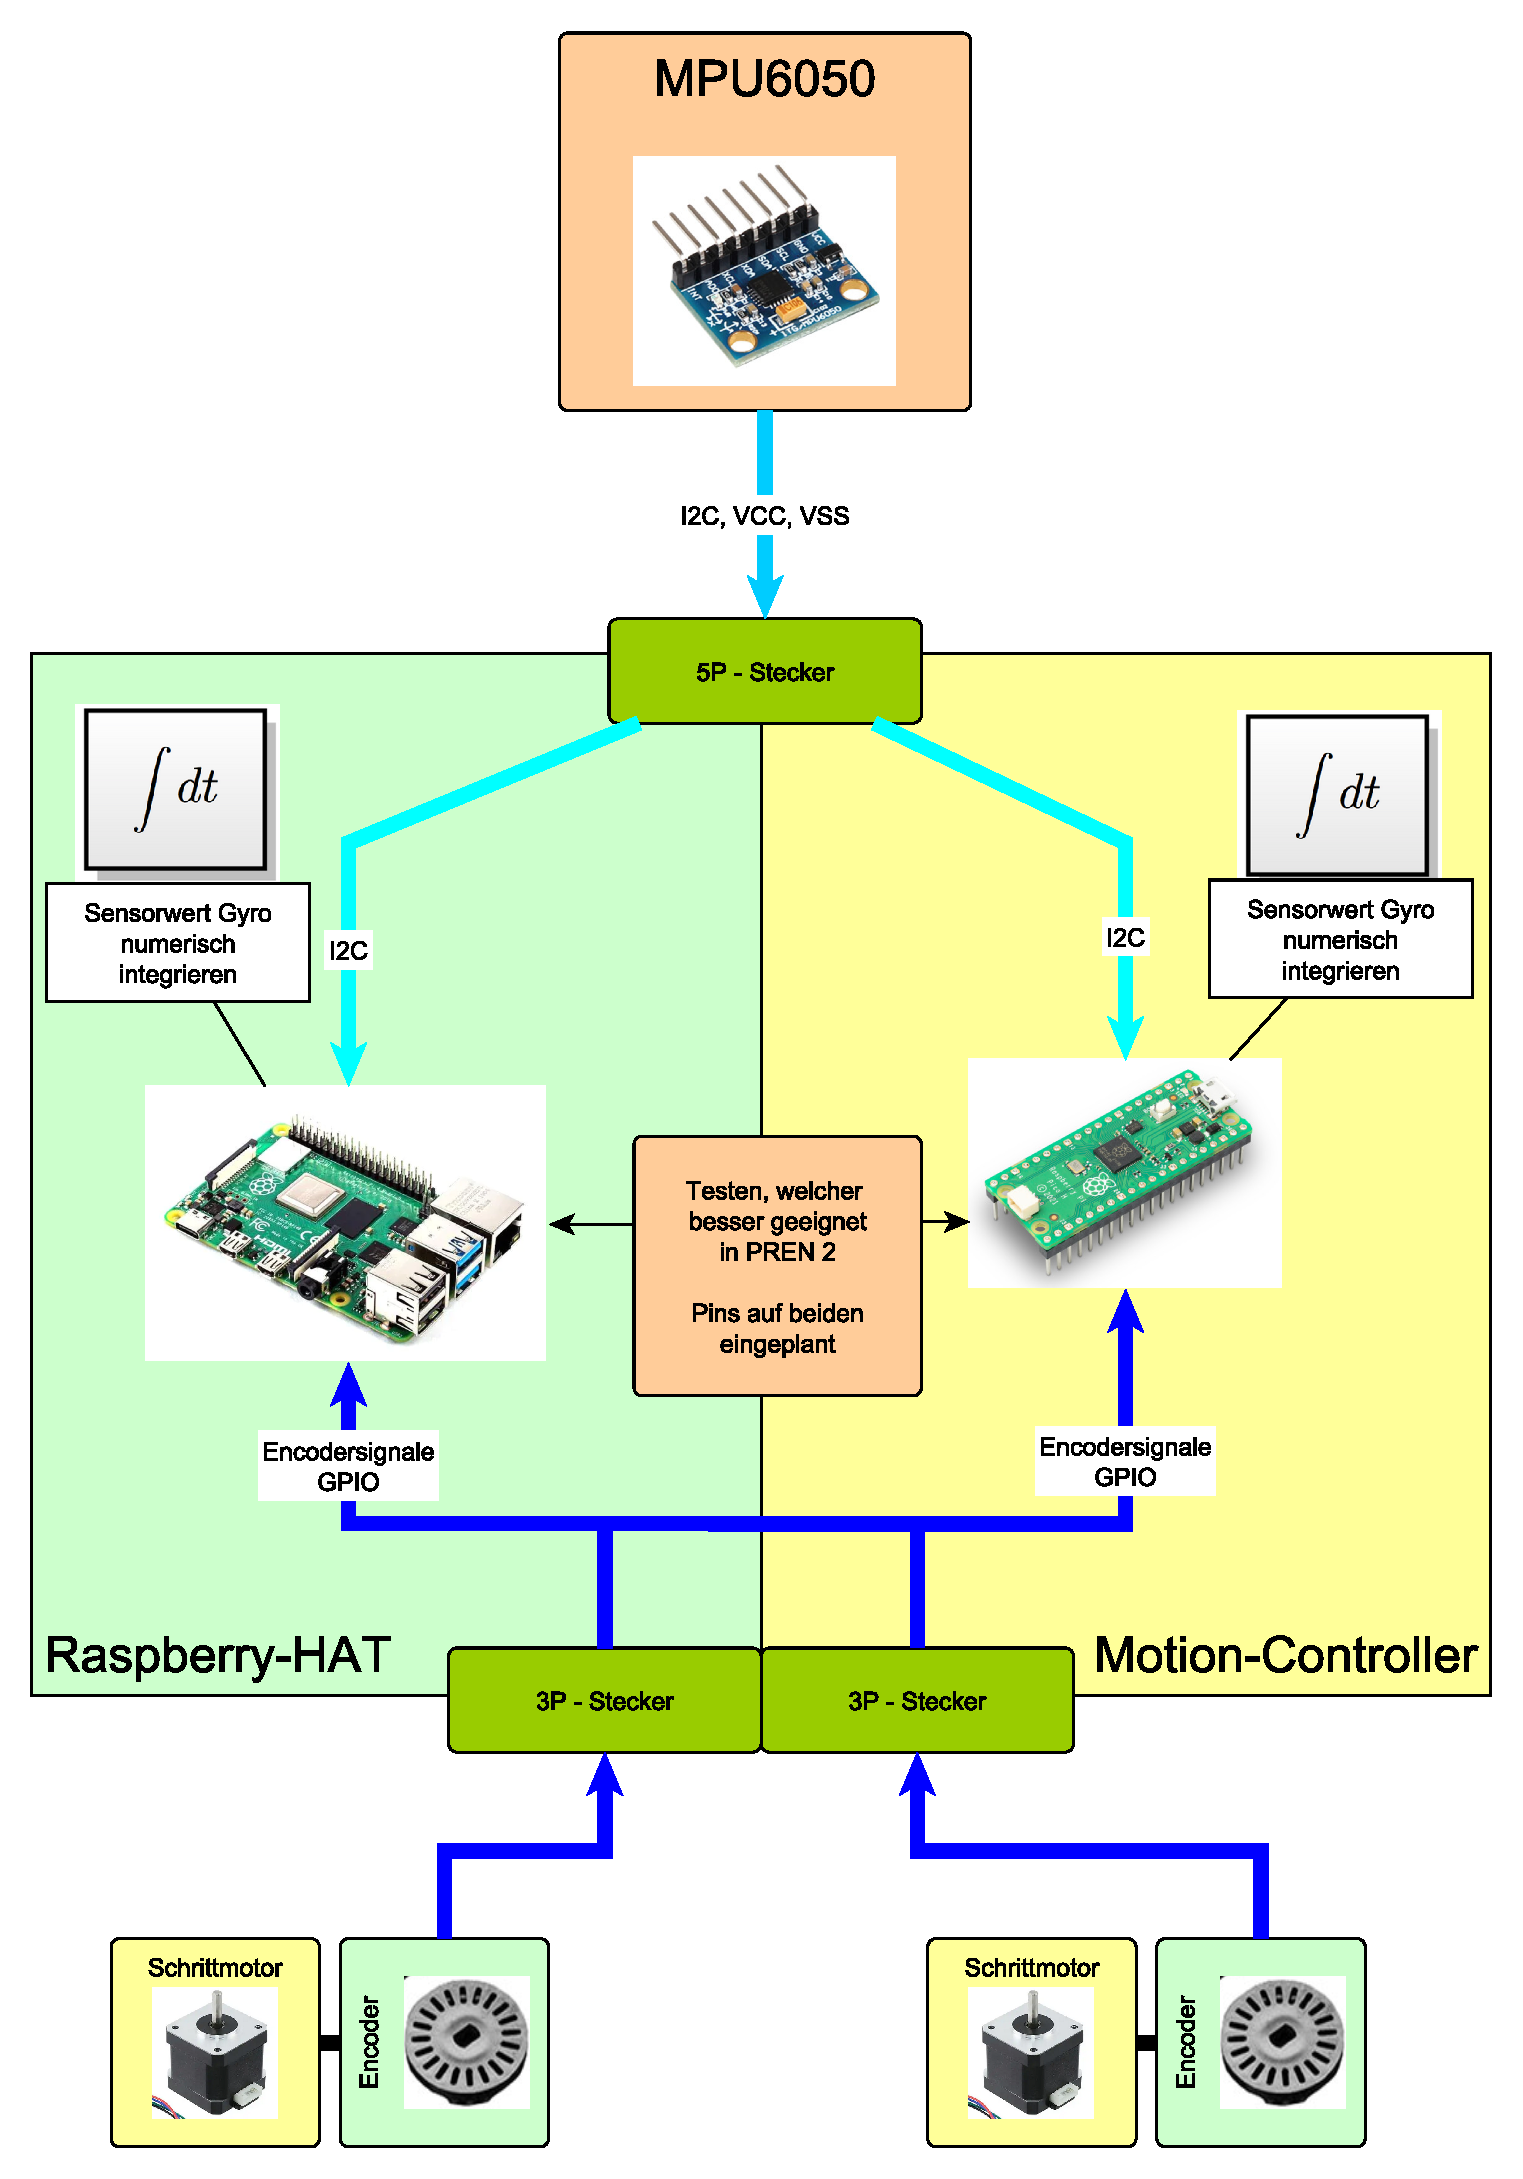
\includegraphics[width=0.75\textwidth]{./fig_Strecke_Tracken/Topologie_MPU6050.pdf}
    \caption{Blockschaltbild Sensorik Streckenrückverfolgung}~\label{fig:Blockschaltbild_StreckenTracken}
\end{figure}

% ===================================================================================
\paragraph{Winkelerfassung}
Der Winkel des Pfadfinders wird, wie in Anhang~\ref{appendix:Strecke_Tracken}
konzeptioniert, über ein Gyroskop ermittelt. Dieses erfasst die Änderungsrate
des aktuellen Winkels zu jeder Zeit und Integriert sie jede $25\mu s$ numerisch
auf. Dadurch kann eine sehr genaue Angabe darüber getroffen werden, in welcher
Orientierung sich das Gerät aktuell befindet.

Mangels Echtzeitfähigkeit ist es nicht sicher, ob der Raspberry Pi in der Lage
ist, das Gyroskop ausreichend genau auszulesen. Deshalb wird ein entsprechender
Steckplatz sowohl auf dem Antriebs-Controller, als auch auf dem Raspberry-HAT
vorgesehen, um dies im Nachfolgemodul PREN2 noch zu testen.

\paragraph{Zurückgelegte Strecke}
Wie in der Konzeption erfwähnt, wird die zurückgelegte Strecke des Pfadfinders
über Encoder ausgezählt. Die Auflösung beträgt

(YANNIK LOCHSCHEIBE).

In einem zweiten Versuch soll im Folgemodul PREN2 getestet werden, ob es
ausreichen könnte, die zurückgelegten Schritte des Schrittmotorentreibers für
diese Referenz zu verwenden. Dieser Versuch kann allerdings erst ausreichend
aussagekräftig durchgeführt werden, wenn ein erster Roboter gebaut ist.

\end{document}